\section{Représentations graphiques}
Illustration de différents diagrammes à partir des données concernant le nombre d'élèves par niveau dans un collège.
$150$ en $6^e$; $200$ en $5^e$; $150$ en $4^e$; $100$ en $3^e$
\subsection{Tableaux}
\begin{remarque}
   Pour \textbf{lire} plus facilement des informations, il est pratique de les \textbf{rassembler} et de les \textbf{organiser} dans un tableau.
\end{remarque}

\Stat[Qualitatif,Tableau,Donnee=Niveau,Effectif=Nombre d'élèves]{$6^e$/150,$5^e$/200,$4^e$/150,$3^e$/100,Total/600}
\subsection{Diagramme en bandes}
\begin{definition}
   Dans un \textbf{diagramme en bandes}, l'\textbf{aire de chaque bande} est proportionnelle à l'effectif qu'elle repr\'esente.
\end{definition}

\begin{center}
   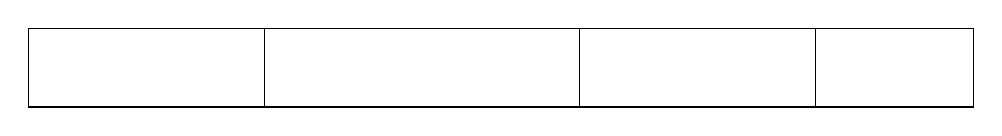
\begin{tikzpicture}
      \coordinate(A) at (2,1);
      \coordinate(B) at (5,1);
      \coordinate(C) at (9,1);
      \coordinate(D) at (12,1);
      \coordinate(E) at (14,1);
      \coordinate(F) at (14,2);
      \coordinate(G) at (12,2);
      \coordinate(H) at (9,2);
      \coordinate(I) at (5,2);
      \coordinate(J) at (2,2);

      \draw (A) -- (E) -- (F) -- (J) -- cycle;
      \draw  (I) -- (B);
      \draw  (H) -- (C);
      \draw  (G) -- (D);
      \tkzLabelSegment[sloped,above](A,B){$6^e$};
      \tkzLabelSegment[sloped,above](B,C){$5^e$};
      \tkzLabelSegment[sloped,above](C,D){$4^e$};
      \tkzLabelSegment[sloped,above](D,E){$3^e$};

   \end{tikzpicture}
\end{center}
\subsection{Diagramme en barres ou diagramme bâtons}
\begin{definition}
Dans un \textbf{diagramme en barres ou en bâtons}, la \textbf{hauteur de chaque barre ou bâton} est proportionnelle à l'effectif qu'elle repr\'esente.
\end{definition}
\begin{center}
\scalebox{0.8}{
   \Stat[%
      Qualitatif,%
      Graphique,%
      Donnee=Niveau,%
      Effectif=Nombre d'élèves,%
      Unitey=0.01,%
      PasGrilley=50,%
      Pasy=100,%
      Unitex=2,%
      Grille,%
      LectureFine%
   ]{$6^e$/150,$5^e$/200,$4^e$/150,$3^e$/100}}
\end{center}
\subsection{Diagramme circulaire ou camembert}
\vspace*{-15mm}
\begin{minipage}{0.8\linewidth}
   \begin{definition}
      Dans un \textbf{diagramme circulaire ou camembert}, l'\textbf{angle de chaque secteur} est proportionnel à l'effectif qu'elle repr\'esente.

      L'effectif total est représenté par \ang{360}.   
   \end{definition}
\end{minipage}
\hspace*{-15mm}
\begin{minipage}{0.2\linewidth}
   \begin{center}
      \scalebox{0.8}{\Stat[Qualitatif,Graphique,Angle,Hachures,AffichageAngle]{$6^e$/150,$5^e$/200,$4^e$/150,$3^e$/100}}
   \end{center}
\end{minipage}

\subsection{Diagramme semi-circulaire}
\begin{minipage}{0.8\linewidth}
   \begin{definition}
   Dans un \textbf{diagramme semi-circulaire}, l'\textbf{angle de chaque secteur} est proportionnel à l'effectif qu'elle repr\'esente.
   \par
   L'effectif total est représenté par \ang{180}.
   \end{definition}
\end{minipage}
\hspace*{-15mm}
\begin{minipage}{0.2\linewidth}
   \begin{center}
      \scalebox{0.8}{\Stat[Qualitatif,Graphique,SemiAngle,Hachures,AffichageAngle]{$6^e$/150,$5^e$/200,$4^e$/150,$3^e$/100}}
   \end{center}
\end{minipage}
   
\subsection{Graphique cartésien}
\begin{definition}
Un graphique cart\'esien permet de repr\'esenter l'\'evolution d'une grandeur \textbf{en fonction} d'une autre.
\end{definition}
\begin{exemple*1}
   \titreExemple{Relevé des températures au cours d'une matinée à Lyon}

   \begin{center}      
      \Stat[Representation,Grille,Graduations,Xmin=0,Ymin=0,Xmax=12,Ymax=12,Xstep=0.8,Ystep=2,%
         PasGrilleX=1,PasGrilleY=2,RelieSegment,LabelX=Heure,LabelY=Températures en \Temp{}]{%
         0/2,1/2,2/1.25,3/1,4/1,5/0.5,6/1,7/2,8/4,9/5,10/8,11/10
      }
   \end{center}
\end{exemple*1}